\section{Introduction}
\label{Introduction}

\begin{wrapfigure}{r}{0.5\columnwidth}
\vspace{-1.6cm}
\begin{center}
{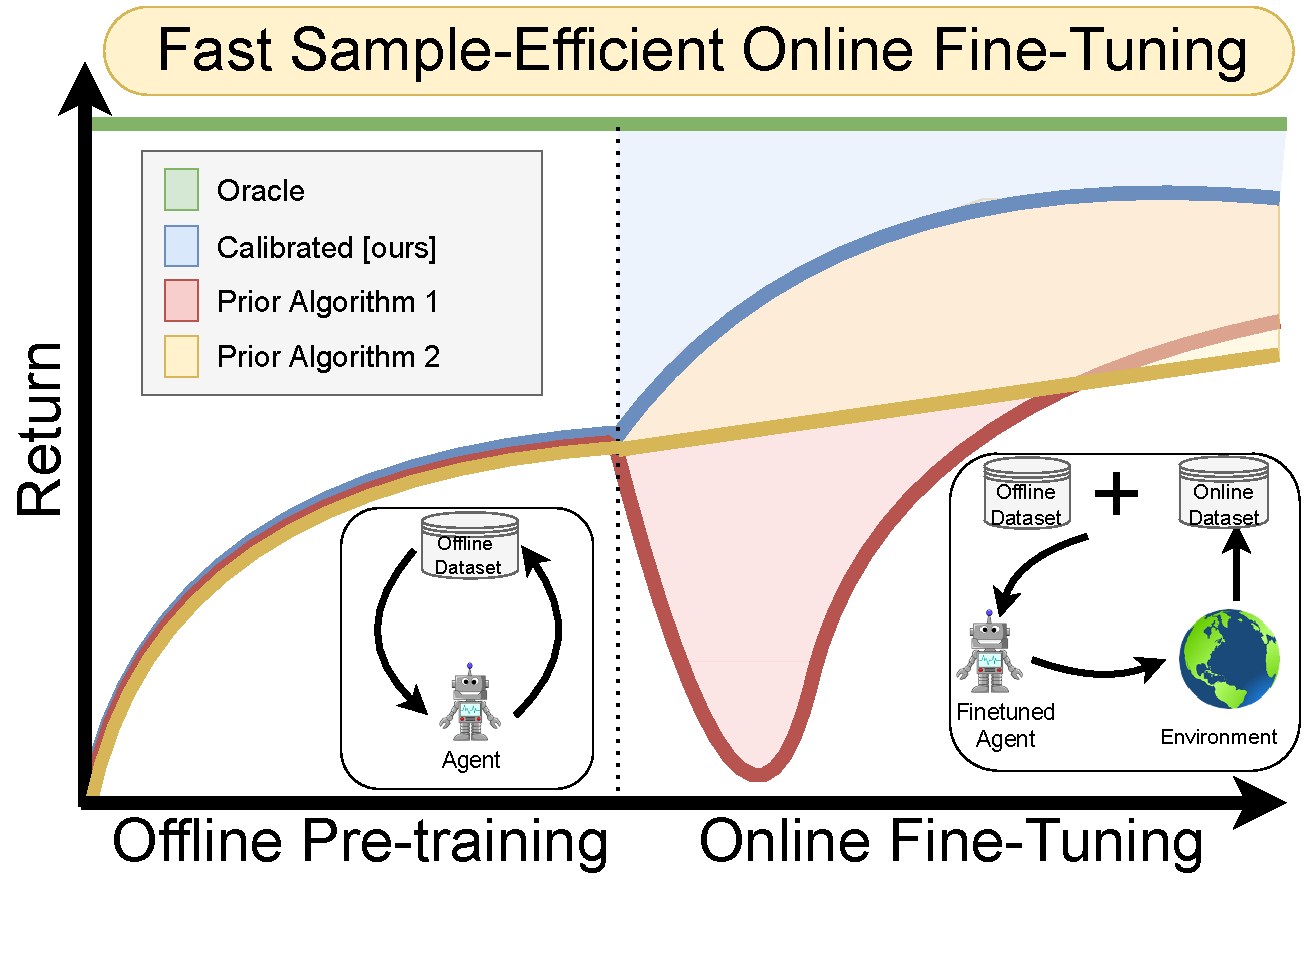
\includegraphics[width=0.85\linewidth]{chapters/cal_ql/figs-sample/Teaser_V2.pdf}}
\vspace{-0.4cm}
\caption{
\footnotesize{We study \textbf{offline RL pre-training followed by online RL fine-tuning}. Some prior offline RL methods tend to exhibit slow performance improvement in this setting (yellow), resulting in worse asymptotic performance. Others suffer from initial performance degradation once online fine-tuning begins (red), resulting in a high cumulative regret. We develop an approach that ``\emph{calibrates}'' the learned value function to attain a fast improvement with a smaller regret (blue).}}
\vspace{-0.7cm}
\label{fig:teaser}
\end{center}
\end{wrapfigure}

Modern machine learning successes follow a common recipe: pre-training models on general-purpose, Internet-scale data, followed by fine-tuning the pre-trained initialization on a limited amount of data for the task of interest~\cite{he2022masked,devlin2018bert}. How can we translate such a recipe to sequential decision-making problems? A natural way to instantiate this paradigm is to utilize offline reinforcement learning (RL) methods~\cite{levine2020offline} for initializing value functions and policies from static datasets, followed by online fine-tuning to improve this initialization with limited active interaction. If successful, such a recipe might enable effective online RL with much fewer samples than current methods that learn from scratch.

Many algorithms for offline RL have been applied to online fine-tuning. Empirical results across such works suggest a counter-intuitive trend: policy initializations obtained from more effective offline RL methods tend to exhibit worse online fine-tuning performance, even within the same task (see Table 2 of~\cite{kostrikov2021offline} \& Figure 4 of \cite{xiao2023the}). On the other end, online RL methods training from scratch (or RL from demonstrations~\cite{vecerik2017leveraging},
where the replay buffer is seeded with the offline data) seem to improve online at a significantly faster rate. But these online methods require actively collecting data by rolling out policies from scratch, which inherits similar limitations to na\"ive online RL methods in problems where data collection is expensive or dangerous. Overall, these results suggest that it is challenging to devise an offline RL algorithm that both acquires a good initialization from prior data and also enables efficient fine-tuning.

How can we devise a method to learn an effective policy initialization that also improves during fine-tuning? Prior work~\cite{kumar2020conservative,cheng2022adversarially} shows that one can learn a good offline initialization by optimizing the policy against a \emph{conservative} value function obtained from an offline dataset. But, as we show in Section~\ref{sec:empirical_analysis}, conservatism alone is insufficient for efficient online fine-tuning. Conservative methods often tend to ``unlearn'' the policy initialization learned from offline data and waste samples collected via online interaction in recovering this initialization. We find that the ``unlearning'' phenomenon is a consequence of the fact that value estimates produced via conservative methods can be significantly lower than the ground-truth return of \emph{any} valid policy. Having Q-value estimates that do not lie on a similar scale as the return of a valid policy is problematic. Because once fine-tuning begins, actions executed in the environment for exploration that are actually worse than the policy learned from offline data could erroneously appear better, if their ground-truth return value is larger than the learned conservative value estimate. Hence, subsequent policy optimization will degrade the policy performance until the method recovers.  
%%AK.5.6: I wonder if we need to show some evidence of the above mechanism to lose the offline initialization in our experiments. It is pretty intuitive to me, but not to everyone for sure...
%%SL.5.7: It's not completely intuitive, but I think it's fine to explain this point in a later section rather than making the intro more complicated. What I do think would be good here though it better phrase "subsequent policy improvement will begin to lose the initialization" -- I think what you mean is that subsequent online policy updates will make the policy worse, but this is confusing because the word "improvement" is overloaded (i.e., it could mean "steps that make the policy better", which is very paradoxical here, or just "updates to the policy")

% Our approach
If we can ensure that the conservative value estimates learned using the offline data are \emph{calibrated}, meaning that these estimates are on a similar scale as the true return values, then we can avoid the unlearning phenomenon caused by conservative methods (see the formal definition in~\ref{cond:calibration}). Of course, we cannot enforce such a condition perfectly, since it would require eliminating all errors in the value function. Instead, we devise a method for ensuring that the learned values upper bound the true values of some \emph{reference policy} whose values can be estimated more easily (e.g., the behavior policy), while still lower bounding the values of the learned policy. Though this does not perfectly ensure that the learned values are correct, we show that it still leads to sample-efficient online fine-tuning. Thus, our practical method, \textbf{calibrated Q-learning} \textbf{(\methodname)}, learns conservative value functions that are ``calibrated'' against the behavior policy, via a simple modification to existing conservative methods.

The main contribution of this paper is \methodname, a method for acquiring an offline initialization that facilitates online fine-tuning. \methodname\ aims to learn conservative value functions that are calibrated with respect to a reference policy (e.g., the behavior policy). Our analysis of \methodname\ shows that \methodname\ attains stronger guarantees on cumulative regret during fine-tuning. In practice, \methodname\ can be implemented on top of conservative Q-learning~\cite{kumar2020conservative}, a prior offline RL method, without any additional hyperparameters. We evaluate \methodname\ across a range of benchmark tasks from \cite{fu2020d4rl}, \cite{singh2020cog} and \cite{AWAC}, including robotic manipulation and navigation. We show that \methodname\ matches or outperforms the best methods on all tasks, in some cases by 30-40\%.

